\documentclass[11pt,letterpaper]{article}
\usepackage{cogsys}
\usepackage{cogsysapa}
\usepackage[utf8]{inputenc}
\usepackage[T1]{fontenc}
\usepackage{times}
\usepackage[pdftex]{graphicx} % use this when importing PDF files

 % First page headings for accepted submissions.
\cogsysheading{X}{20XX}{X-X}{4/2015}{X/20XX}
 % First page headings for poster submissions.
%\cogsysposterheading{First}{2012}{1-18}

\ShortHeadings{Interactive Reasoning to Solve Knowledge Goals}
              {B.\ Bengfort and M.\ Cox}

\begin{document}

\title{Interactive Knowledge-Goal Reasoning}

\author{Benjamin Bengfort}{bengfort@cs.umd.edu}
\address{Department of Computer Science, University of Maryland,
         College Park, MD 20742 USA}
\author{Michael Cox}{michael.cox@wright.edu}
\address{Wright State Research Institute,
         Beavercreek, OH 45431 USA}
\vskip 0.2in

% Title (1000 readers)
% Abstract (4 sentences, 100 readers)
% Introduction (1 page, 100 readers)
% The problem (1 page, 10 readers)
% My idea (2 pages, 10 readers)
% The details (5 pages, 3 readers)
% Related work (1-2 pages, 10 readers)
% Conclusions and further work (0.5 pages)

\begin{abstract}
Knowledge goals are used by reasoning entities to fill-in information required for decision making and are an important part of computational understanding systems. Simple knowledge goals can be solved through traditional information retrieval techniques or database queries. In order to solve complex knowledge goals, however, a plan must be composed and executed in an investigative manner. During computational investigation, goals of both the system and the user can change, resulting in goal trajectories that may inform future goal solutions. In this paper, we propose an interactive reasoning system that leverages a case-based methodology to solve complex knowledge goals represented as natural language queries.
\end{abstract}

\section{Introduction}

A \textit{knowledge goal} represents the purposeful need to acquire information in order to fill-in gaps of world knowledge for a reasoning entity or to extend the database of a computational understanding system \cite{ram_goal-based_1991}. For humans, knowledge goals are most easily represented as questions, and current research on dialog-driven question and answer systems focus on the semantic parsing of a natural language question to a structured database query \cite{yahya_natural_2012} or lambda calculus representation \cite{berant_semantic_2013}. These parsing approaches are making headway in the solution of simple knowledge goals, where the primary task is a retrieval from some structured knowledge base; especially goals that ask “who”, “what”, “when”, or “where”. This approach, however, cannot solve complex knowledge goals including aggregations, opinions (recommendations), or explanations for “why” or “how” questions. As a result, even though information retrieval (IR) systems and search have made information easily accessible, there has been the growth of community-driven question sites such as Quora \cite{wang_wisdom_2013} to connect users to the more complex answers they are looking for.

Humans solve complex knowledge goals through \textit{investigation}, dividing harder questions into simpler sub-knowledge goals whose solutions are more easily obtained. When solving knowledge goals, humans also take into account context and approach new problems by leveraging techniques that have worked in the past. A system that models how humans investigate questions will \textit{deconstruct} a complex goal, \textit{integrate} relevant knowledge, and \textit{resuse} methods of investigation. Investigation can be represented as a plan to solve the larger knowledge goal, and if the tasks or subgoals of knowledge acquisition plans are simple knowledge goals that can be solved via structured data retrieval, then a system can be said to compute complex knowledge goals through a planning process that involves the purposeful combination of simpler knowledge goals.

In this paper we present the vision for an interactive knowledge goal reasoning system that uses a case-based reasoning (CBR) methodology to deconstruct complex knowledge goals based on previous cases for similar questions. The system will provide users with goal-driven solutions to natural language queries by proposing plans of simpler knowledge goals, the aim of which are computationally tractable tasks like database queries or document retrieval. The system takes into account the context of the goal by leveraging semantic resources applied to the question and utilizes a wide array of data sources to perform retrieval tasks - from database queries, to search, to providing other user responses for complex questions. As subtasks are selected by the initiating user, the CBR system reinforces and indexes how the plan was solved in order to provide more relevant plans or responses in the future.

Because this type of system is interactive and adaptive it is subject to goal changes, where the original knowledge goal is changed or refined slightly while the user interactively follows a solution plan. The complete case for solving a complex knowledge goal therefore represents a \textit{goal trajectory}. Goal trajectories are important for refining future cases, ranking plan solutions, and having the system anticipate knowledge goals to propose better plans. Furthermore, the combination of goal trajectories can be seen as a creative process, leading to the extension of not only the case base - but also to automatically extend the knowledge base of the system.

%% Should I add the components (concept, task, context) of the question to the introduction?

In order to explore interactive knowledge goal reasoning, we will first discuss knowledge goals and goal trajectories in detail. This discussion will lead to a brief taxonomy of questions, which is vital to understanding the many types of cases in a natural language query system. In the second section, we will describe our proposed case based methodology, including the casebase representation, acquisition, and management. Finally we will present three applications or case studies that demonstrate how an interactive knowledge goal reasoning system might be employed.

\section{Knowledge Goals}

In information retrieval (IR) systems, the input is a query that usually takes the form of a boolean combination of keywords and the expected output is a ranked list of documents that have a high relevance to the keyword combination. Similarly in database management systems the input is a formal query that must conform to the logical structure of the information, and the output is a set of records or aggregations that also conform to the schema. While these systems are important in the management of large-scale, multi-modal information sets, they do not represent the way that humans formulate knowledge goals: questions. Although search and structured database queries may be viewed as stand-ins for knowledge goals, they only embed the execution context or \textit{task} of the knowledge goal, whereas natural language queries express more information related to the goal and can be both \textit{simple} and \textit{complex} where formal languages are not as flexible.

We can define \textit{simple} knowledge goals as questions that are directly tied to a retrieval task and whose solution may be either traditional information retrieval or structured queries. Consider the question ``\textit{Who won the World Cup?}'' The goal of this question is to determine the \texttt{Country} entity that won the most recent World Cup and possibly also the \texttt{Result} in the form of the competing teams and final score. Search methodologies would find documents with a high relevance to the tokens in the text of the question - particularly ``World Cup''. A structured database query upon some knowledge base would require semantic parsing to determine look up the relationship between the \texttt{FIFA World Cup} topic, and a specific \texttt{Country} topic. Even with these challenges, the result of both search and database query would fulfill the knowledge goal.

\textit{Complex} knowledge goals, on the other hand, cannot be solved simply through a single retrieval task and are generally related to questions that require investigation, opinion, explanation, or knowledge generation. Consider the question ``\textit{Where should I go to dinner?}'' This question is not a simple retrieval task because there is no database entry or set of relevant documents that might help solve the goal of determining a restaurant to eat the evening meal. Moreover, this routine question will have different responses when asked by the same user multiple times, depending on context like geographic location, the season, or changing user preferences. Other complex knowledge goals are used to generate information, for example ``\textit{Can a crocodile complete a steeplechase?}'', a fact that is probably not part of most knowledge bases. Unless someone has already investigated this question, the goal will have to be decomposed into lines of questioning related to the physical requirements of completing a steeplechase compared to the athletic ability of crocodiles.

% Do we need more here?

\subsection{Knowledge Goal Composition}

Knowledge goals are composed of three primary components: a set of \textit{concepts}, a \textit{task}, and a specific \textit{context}. In order to create a plan to solve a knowledge goal, a computational system must first identify and parse these components. Each component contributes to the solution as follows:

\begin{enumerate}

\item \textbf{Concept}: The knowledge goal is relevant to a specific set of structured semantic concepts, both entities and predicates, which are either directly specified or implied. The concept of the question identifies the domain of the query plan as well as the expected response.

\item \textbf{Task}: The task indicates the purpose of the question and is usually implied in a natural language query and related to the motivation of the questioner. For example, in the case of simple knowledge goals the task may be search or database query; for more complex knowledge goals the task may be explanation or knowledge generation. It is by task that different types of knowledge goals are categorized in the taxonomy below.

\item \textbf{Context}: Knowledge goals are not specified in isolation, but are directly related to the questioner and as such must be considered in relation to their context. Contextual information includes temporal, geographic, and preference information and is essential for plan refinement and to resolve ambiguity.
\end{enumerate}

In the question ``\textit{When is the next flight to Paris?}'' the \textit{concept} explicitly includes the topic \texttt{Air Travel} as well as a city, \texttt{Paris}. Implied concepts might include \texttt{Paris, France}, the most popular city named Paris, and \texttt{Charles de Gaulle Airport}. The \textit{task} can generally be defined as a simple database query or search, but more specifically the return of a specific \texttt{Flight} record. The \texttt{context} is critical as well, especially the geographic context (the next flight to Paris from the city where the user is currently located) and the temporal context (in order to determine when the next flight might be).

Many applications simplify one or more components of a knowledge goal in order to be effective. Domain-specific applications reduce ambiguity in concepts and context by only allowing specifically relevant knowledge goals. More commonly, applications simplify the task - designed to return only a single type of result. However, as users are utilizing mobile devices to provide even more contextual clues to applications and with the wide spread availability of large, general knowledge bases applications which generalize question and answer systems are becoming more tractable.

\subsection{Solving Knowledge Goals}

% Mention interactivity? %

An important step in the development of dialog-driven question and answer systems was the creation of large-scale structured knowledge bases like Freebase \cite{bollacker_freebase:_2008} or Yago2 \cite{suchanek_yago:_2007}. These databases represent a wealth of information generated from collaboratively edited encyclopedic sites like Wikipedia and provide the means with which to make factual queries about the world. Semantic parsers can take advantage of hierarchical, relational ontologies which allow for a generalization in the domain or \textit{concept} component of a question. For simple knowledge goals, semantic parsers can transform natural language questions into structured queries like SPARQL or SQL \cite{yahya_natural_2012}, a lambda-calculus representation \cite{berant_semantic_2013}, or simply a template from which to directly search other answers \cite{unger_template-based_2012}.

However, these parsers will struggle even with slightly more complex natural language queries whose task is a database lookup in a knowledge base, for example ``\textit{Who was the King of England when Thomas Jefferson was President?}'' This knowledge goal is a factual retrieval that can be solved through a chain of sub knowledge goals to first solve which years Thomas Jefferson was President of the United States, then using the result from that query to determine the King of England during that time period. Similarly, knowledge goals that require aggregation such as ``\textit{How many countries have won three consecutive gold medals in a single sport?}'' may be able to to be transformed into a series of simpler sub queries which contribute information to a final result.

The decomposition method of solving fact-based retrieval questions can also be applied to complex knowledge goals whose task is not simply a query or search. When a complex knowledge goal is reduced to one or more simpler sub goals, the result is a hierarchical plan to solve the original knowledge goal. If the final tasks of such a plan are simple knowledge goals which can be transformed into a query or a search, then a system can said to solve complex knowledge goals through the computationally tractable combination of simpler knowledge goals.

\begin{figure}
	\centering
	    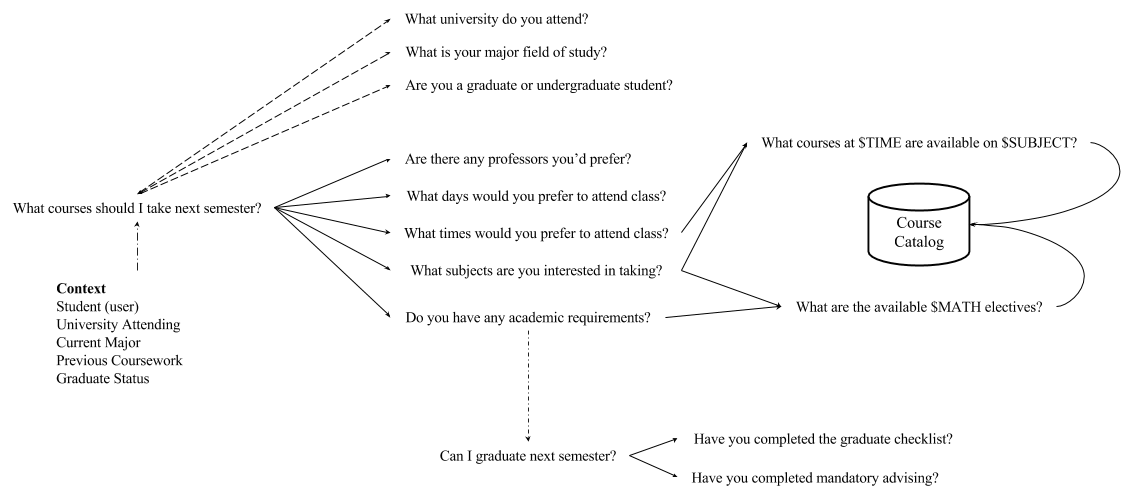
\includegraphics[width=\textwidth]{figures/simple_trajectory.png}
    \caption{\label{fig:simple_trajectory.png}A complex knowledge goal solution with trajectory change.}
\end{figure}

Consider an example complex knowledge goal, ``\textit{What courses should I take next semester?}'', outlined in Figure \ref{fig:simple_trajectory.png}. This knowledge goal is routine, executed by the same user on a regular interval and common enough that a casebase of solutions is readily available. The task of this knowledge goal is to create a list of courses which are available next semester and which the student will presumably be able to register for. The concept of the question is explicitly the domain of courses that are available at a particular university during a particular semester. The context for a user determines preference in terms of the selected major or course level as well as geographical context (which specific university) and temporal context (which specific semester).

In order to solve this knowledge goal, a plan of simpler sub knowledge goals may be offered to the user. If contextual information is missing, the system might respond with ambiguity resolution goals of its own (e.g. ``\textit{Have you selected a major?}''). Otherwise simpler sub knowledge goals could include ``\textit{What days and times would you prefer?}'', ``\textit{Are there any academic subjects you're interested in?}'', or ``\textit{Do you have any academic requirements?}'' Responses to these sub-knowledge goals would lead to even simpler knowledge goals which can be eventually be queried against a course catalog, ``\textit{What Economics courses are available on Monday and Wednesday?}''

\subsection{Goal Trajectories}

The solution to complex knowledge goals is an interactive reasoning approach where a complex knowledge goal is broken down into a hierarchical plan of simpler sub goals and tasks. However, both plans and knowledge goals are adaptable and subject to change as a system and user proceeds in executing simpler goals \cite{munoz-avila_case-based_2008}. When the original knowledge goal plan adapts during the execution of a knowledge goal, the path that led to the solution of the new knowledge goal is represented by a goal trajectory.

Goal trajectories can be influenced by other users in the system, either humans who are issuing similar queries and providing recommended goals through collaborative filtering \cite{hayes_case-based_2001} or via monitoring of automatic systems on new information or relevant data that has been added to the knowledge base. In either case, goal changes can be seen as a planning problem that must be responsive to change \cite{cox_mixed-initiative_2007}. Goal trajectories also explicitly define relationships between knowledge goals that can be used as cases for future solutions.

In the example from Figure \ref{fig:simple_trajectory.png}, a goal trajectory is demonstrated by the proposed sub-knowledge goal, ``\textit{Do you have any academic requirements}'', which leads the user to adapt the goal to ``\textit{Can I graduate next semester}''

\subsection{Knowledge Goal Taxonomy}

In the next section, we will discuss the solution of knowledge goals by decomposing a complex knowledge goal in to subsequently simpler knowledge goals. However, in order to determine an execution plan for knowledge goals, some idea of the types of knolwedge goals that might be in a system as well as their relative complexity is required. Knowledge goals as described in \cite{ram_knowledge_1990} are presented with a categorization based on the task that they arise from. Similarly, we will extend this taxonomy with our planning framework, given the components of a knowledge goal discussed in the last section.

\subsubsection{Simple Knowledge Goals}

The simplest knowledge goals should be computationally tractable such that they can be solved with a minimal amount of user involvement. Simple knowledge goals have tasks that range from search to database queries to computational tasks like parsing, aggregation, or inference. In an \textit{interactive} system, both users and the system have simple knowledge goals. The system uses knowledge goals to resolve ambiguity through dialog boxes or through other types of feedback.

\begin{enumerate}

\item \textbf{Textual}: Questions related to both semantic or syntactic analysis of text, usually as a response to ambiguity. Tasks related to text questions include anaphora resolution or word sense disambiguation. Users may ask to define a word, the system may ask to clarify a concept.

\item \textbf{Contextual}: Questions designed to specify the result of a knowledge goal according to the user's context in terms of preference, geography, or time. Similar to textual questions, these types of questions are "meta-questions" that are used to tailor the execution of a knowledge goal solution.

\item \textbf{Rhetorical}: Questions that should not return an answer. Questions that are used as placeholders or to express frustration are important to identify as simple knowledge goals because they identify terminal tasks in question plans.

\item \textbf{Retrieval}: Questions that expects a single fact returned from the database and may be transformed into a structured query. These types of questions may perform aggregations or filtering upon the knowledge base, but typically only return a single result or a small list of results.

\item \textbf{Search}: Questions that require a larger scope or domain and whose expected results are a list of relevant documents.

\end{enumerate}

The tasks related to these simple knowledge goals are all able to be computed on behalf of a user. Knowledge goals that fall into these categories are the simplest goals that may be involved in an interactive knowledge goal reasoning system.

\subsubsection{Complex Knowledge Goals}

Complex knowledge goals must be reasoned upon rather than computed directly, and cannot be directly parsed into a executable representation. Instead, a plan must be developed in order to solve complex knowledge goals which leverages the context and concepts in the goal. The types of tasks for complex knowledge define the categorization of these goals as follows:

\begin{enumerate}

\item \textbf{Explanation}: Questions that require an explanation and return an explanatory data structure. Tasks include the detection and resolution of anomalies as well as the construction of an inferential or causal explanation.

\item \textbf{Relevance}: These questions are designed to expand the current knowledge framework by adding relevance links between questions and related entities, answers or other questions. Relevance can be used in later processing as a shortcut to retrieval from a casebase.

\item \textbf{Socratic}: Socratic questions return a question as an answer, or rather a plan that consists of knowledge goals that are designed to answer the larger question.

\item \textbf{Research}: These types of questions are designed to add information to a knowledge base, either by adding facts or creating knowledge from other knowledge sources. The system should identify research questions based on unsatisfactory queries and add them to the system for later investigation.

\item \textbf{Routine}: Questions that are routine are asked frequently or on a specific interval, however the required answer will differ based on the context or timing of the question and will most likely not return the same answer as a previous instance of the question.

\end{enumerate}

Tasks related to solving complex knowledge goals require some learning framework to mimic how humans solve similar goals. In an interactive reasoning system, the learning framework can include the use of similar cases or solutions to goals to propose a plan to solve the complex goal, or to connect related users as they investigate similar goals.

\section{Case Based Methodology}

\begin{figure}
	\centering
	    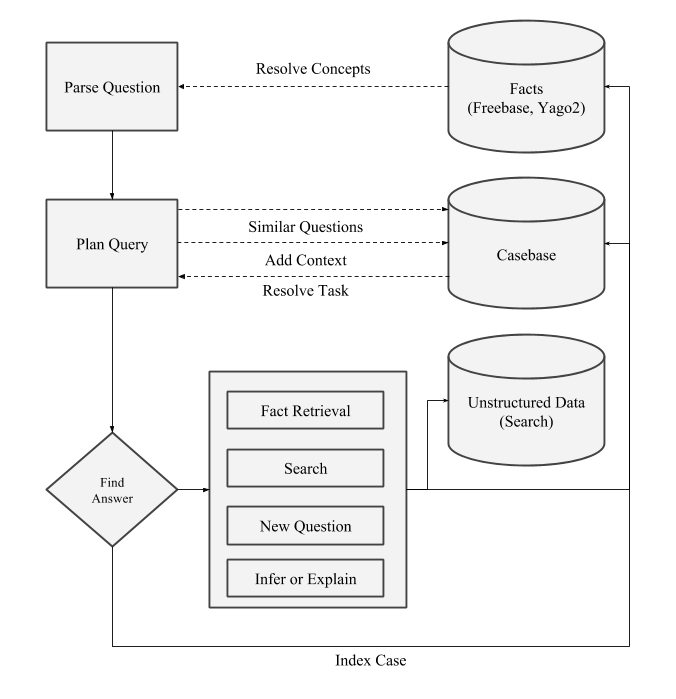
\includegraphics[width=0.5\textwidth]{figures/architecture.png}
    \caption{\label{fig:architecture.png}An architecture for interactive knowledge goal reasoning.}
\end{figure}

\subsection{Case Representation}

\subsection{Case Acquistion}

\subsection{Case Management}

\section{Case Studies and Applications}

In order to acquire a casebase with which to study question and answer systems in the context of goal trajectories, we propose to use the Kyudo application to allow users to generate a dataset of their own goals, questions, and answers.

Users will be asked to participate in one or more of three ``tasks'' or scenarios that have been developed to guide casebase acquisition. The users should specifically identify which scenario they are participating in when they use the system.


\subsection{Conceirge}

Concierge staff are expected to be available to answer questions from tourists who are unfamiliar with the city that they are staying in. Often, they go much further than simple responses to questions such as ``\textit{How do I get to the Eiffel Tower?}'' - they suggest places to eat, other interesting things to see, or warn of “tourist traps” and generally work to not only answer the question that is being asked, but to identify the larger goals of the travelers in order to make their stay excellent.

In this task, the users of the system are expected to ask questions as though they are travelers speaking to a concierge. Other users will then respond to the questions as though they are a concierge, giving tips, feedback, suggestions, recommendations in addition to answering the primary question. In order to make this easy, frame the questions as though you are in a hotel in downtown Washington D.C..

\subsection{Presidential Briefer}

The role of the presidential briefer is to prepare a report on the days news and other intelligence activities to be reported to POTUS first thing in the morning. The goal is to deliver as much information in a short amount of time. As such, the briefer must anticipate the questions that the president might have and prepare answers from them quickly. The final product is the ``brief book'' - a book with an executive summary, then detailed information designed to respond to questions.

In this task, users of the system are expected to anticipate questions that the president might ask when they brief him, specifically from news stories that they are preparing the briefing for. Users should prepare questions and ask them on Kyudo from specific news stories, and include the news stories as background in the details section of the question. ``Answers'' to these questions should be detailed, and also anticipatory of ``follow-on'' questions that the president might ask.

\subsection{Undergraduate Adviser}

Undergraduate advisers must have a large amount of domain specific knowledge from University policy, to course requirements and schedules, to assistance in a realm of domains. They not only answer questions that undergraduates pose to them, but also respond with detailed, specific instructions for the student to carry out.

In this task, the questions will be as from an undergraduate to the adviser - to include issues about courses, plans of study, policy (medical leave, absence, etc.) as well as more personal issues. The answers should be detailed, specific instructions regarding the University policy with clear tasks to carry out.

\section{Related Work}

Systems that leverage large data sets of community organized questions and answers focus on the task of question similarity. Statistical models based on both the question text as well as the answers are discussed in \cite{jeon_finding_2005,jeon_finding_2005-1}, work that culminates in a statistical model for retrieval of answers based on query-similarity likelihoods \cite{xue_retrieval_2008}. Answer selection or ranking from the retrieval is typically based on heuristic methods, especially reputation-based mechanisms where other users evaluate answers directly \cite{wang_wisdom_2013}. Original natural language knowledge navigation used case-based reasoning to direct user queries to FAQ files as in \cite{hammond_faq_1995,burke_question_1997,burke_natural_1997}. While these systems engage users collaboratively to explore questions that are not easily answered by the simple retrieval of documents or require explanations, they are of very little use to artificial cognitive agents.

On the other end of the spectrum, there has been work designed to translate natural language queries directly to a structured query that can operate on fact based semantic knowledge bases, usually into a SPARQL query as in \cite{yahya_natural_2012,unger_template-based_2012} and \cite{berant_semantic_2013}. These automatic approaches rely heavily on semantic disambiguation and entity resolution, evaluating the query itself against the knowledge base \cite{zheng_entity_2012}. Other approaches include the derivation of proto-queries directly from the knowledge base \cite{frank_question_2007} akin to question indexing a structured data set. Retrieval mechanisms like predictive annotation and type coercion have led to the success of Watson and other agent-based knowledge systems \cite{prager_question_2006,kalyanpur_leveraging_2011}. However, these systems are restricted only to the retrieval of facts from a database and usually perform little inference or planning concerning the query.

To date, most of the study to the solution of knowledge goals have focused on either the individual user to parse natural language queries into structured database queries, or upon an artificial agent using machine learning or logic based approaches to infer or guess at missing knowledge. Although there are many automated information extraction processes that can deal with large amounts of data, these processes are susceptible to inconsistencies and rely on raw data - they cannot make inferences or leaps that are not in the data.

\section{Conclusion}

In this paper we have briefly presented a high-level taxonomy of knowledge goals: simple and complex and proposed a representation composed of the concept, task, and context to be used in a case-based interactive reasoning system. We've also shown that reasoning systems must be adaptive and responsive to change to mimic human investigative processes, leading to creativity by allowing for knowledge goal trajectories. For our upcoming research, we are currently building a system that allows the collection of knowledge goal cases, in order to pursue research on cognitive systems of investigation.

% \newpage

% \begin{acknowledgements}
% \noindent
% % Please place your acknowledgements in an unnumbered section at the
% % end of the paper. Typically, this will include thanks to reviewers
% % who gave useful comments, to colleagues who contributed to the ideas,
% % and to funding agencies or corporate sponsors that provided financial
% % support.
% \end{acknowledgements}

\vspace{-0.25in}

{\parindent -10pt\leftskip 10pt\noindent
\bibliographystyle{cogsysapa}
\bibliography{kgworkshop}

}

% Leave a blank line before the closing brace to ensure the final
% reference has the proper indentation.

\end{document}
